% Desenvolvido por Prof. Dr. David Buzatto
%
% Baseado na documentação do abntex2 e nos modelos em
% Microsoft Word propostos pela Profa. Dra. Rosana F. L. Rodrigues
% e pela bibliotecária M.Sc. Maria Carolina Gonçalves do campus
% São João da Boa Vista do IFSP.
%
% Versão 1.3
% Data: 09/08/2018

\documentclass[
	% -- opções da classe memoir --
	article,			% indica que é um artigo acadêmico
	11pt,				% tamanho da fonte
	oneside,			% para impressão apenas no recto. Oposto a twoside
	a4paper,			% tamanho do papel. 
	% -- opções da classe abntex2 --
	chapter=TITLE,		% títulos de capítulos convertidos em letras maiúsculas
	section=TITLE,		% títulos de seções convertidos em letras maiúsculas
	%subsection=TITLE,	% títulos de subseções convertidos em letras maiúsculas
	%subsubsection=TITLE % títulos de subsubseções convertidos em letras maiúsculas
	% -- opções do pacote babel --
	english,			% idioma adicional para hifenização
	brazil,				% o último idioma é o principal do documento
	sumario=tradicional
]{abntex2}


% ---------------------------------------------------------------------------------
%                                   PACOTES
% ---------------------------------------------------------------------------------

% ---
% Pacotes básicos 
% ---
\usepackage{lmodern}			% Usa a fonte Latin Modern
\usepackage[T1]{fontenc}		% Selecao de codigos de fonte.
\usepackage[utf8]{inputenc}		% Codificacao do documento (conversão automática dos acentos)
\usepackage{indentfirst}		% Indenta o primeiro parágrafo de cada seção.
\usepackage{nomencl} 			% Lista de simbolos
\usepackage{color}				% Controle das cores
\usepackage{graphicx}			% Inclusão de gráficos
\usepackage{microtype} 			% para melhorias de justificação
\usepackage{hyperref}
\usepackage{subfig}
\usepackage{epigraph}
\usepackage{url}
\usepackage{placeins}
\usepackage{multirow}
\usepackage[figuresright]{rotating}
\usepackage{chemfig}
\usepackage{amsmath}
\usepackage{amssymb}
\usepackage{enumitem}
\usepackage{bigints}
\usepackage{listings}
\usepackage{tabularx}
\usepackage{booktabs}
\usepackage{etoolbox}
% ---

% ---
% Pacotes adicionais, usados apenas no âmbito do Modelo Canônico do abnteX2
% ---
\usepackage{lipsum}				% para geração de dummy text
% ---

% ---
% Pacotes de citações
% ---
\usepackage[brazilian,hyperpageref]{backref}	 % Paginas com as citações na bibl
\usepackage[alf,abnt-emphasize=bf]{abntex2cite}  % Citações padrão ABNT


% ---------------------------------------------------------------------------------
%                          CONFIGURAÇÕES DOS PACOTES
% ---------------------------------------------------------------------------------

% ---
% Configurações do pacote backref
%
% Para desativar, tire o comentário de \begin{comment} e \end{comment} 
% das próximas linhas e comente a linha \usepackage[brazilian,hyperpageref]{backref}
% acima.
% ---

%\begin{comment}
% ---
% Configurações do pacote backref
% Usado sem a opção hyperpageref de backref
\renewcommand{\backrefpagesname}{Citado na(s) página(s):~}
% Texto padrão antes do número das páginas
\renewcommand{\backref}{}
% Define os textos da citação
\renewcommand*{\backrefalt}[4]{
	\ifcase #1 %
	Nenhuma citação no texto.%
	\or
	Citado na página #2.%
	\else
	Citado #1 vezes nas páginas #2.%
	\fi}%
% ---
%\end{comment}


% listagens
\definecolor{corComentario}{RGB}{150,150,150}
\definecolor{corString}{RGB}{206,123,0}
\definecolor{corPalavraChave}{RGB}{0,0,230}

\lstset{
	numbers=left,
	stepnumber=1,
	firstnumber=1,
	numberstyle=\footnotesize,
	extendedchars=true,
	breaklines=true,
	lineskip=0pt,
	frame=tb,
	basicstyle=\ttfamily\footnotesize,
	showstringspaces=false,
	stringstyle=\color{corString},
	commentstyle=\color{corComentario},
	keywordstyle=\color{corPalavraChave}
}

\newcolumntype{Y}{>{\centering\arraybackslash}X}

\newcommand{\ano}[1]{\def \oano {#1}}
\newcommand{\imprimirano}{\oano}

\newcommand{\mes}[1]{\def \omes {#1}}
\newcommand{\imprimirmes}{\omes}

\newcommand{\dia}[1]{\def \odia {#1}}
\newcommand{\imprimirdia}{\odia}

\newcommand{\area}[1]{\def \aarea {#1}}
\newcommand{\imprimirarea}{\aarea}

\newcommand{\aluno}[1]{\def \oaluno {#1}}
\newcommand{\imprimiraluno}{\oaluno}

\newcommand{\gradorientador}[1]{\def \agradorientador {#1}}
\newcommand{\imprimirgradorientador}{\agradorientador}

\newcommand{\instgradorientador}[1]{\def \ainstgradorientador {#1}}
\newcommand{\imprimirinstgradorientador}{\ainstgradorientador}

\newcommand{\posorientador}[1]{\def \aposorientador {#1}}
\newcommand{\imprimirposorientador}{\aposorientador}

\newcommand{\instposorientador}[1]{\def \ainstposorientador {#1}}
\newcommand{\imprimirinstposorientador}{\ainstposorientador}

\newcommand{\docorientador}[1]{\def \odocorientador {#1}}
\newcommand{\imprimirdocorientador}{\odocorientador}

\renewcommand{\coorientador}[1]{\def \ocoorientador {#1}}
\renewcommand{\imprimircoorientador}{\ocoorientador}

\newcommand{\gradcoorientador}[1]{\def \agradcoorientador {#1}}
\newcommand{\imprimirgradcoorientador}{\agradcoorientador}

\newcommand{\instgradcoorientador}[1]{\def \ainstgradcoorientador {#1}}
\newcommand{\imprimirinstgradcoorientador}{\ainstgradcoorientador}

\newcommand{\poscoorientador}[1]{\def \aposcoorientador {#1}}
\newcommand{\imprimirposcoorientador}{\aposcoorientador}

\newcommand{\instposcoorientador}[1]{\def \ainstposcoorientador {#1}}
\newcommand{\imprimirinstposcoorientador}{\ainstposcoorientador}

\newcommand{\doccoorientador}[1]{\def \odoccoorientador {#1}}
\newcommand{\imprimirdoccoorientador}{\odoccoorientador}

\newcommand{\campus}[1]{\def \ocampus {#1}}
\newcommand{\imprimircampus}{\ocampus}

\newcommand{\grau}[1]{\def \ograu {#1}}
\newcommand{\imprimirgrau}{\ograu}

\newcommand{\curso}[1]{\def \ocurso {#1}}
\newcommand{\imprimircurso}{\ocurso}

% ---
% Informações de dados para cabeçalho
% ---

\instituicao{Instituto Federal de Educação, Ciência e Tecnologia de São Paulo}
\campus{São João da Boa Vista}

\curso{Nome do Curso}
\grau{Definição do grau}

%exemplos
%\curso{Tecnologia em Sistemas para Internet}
%\grau{Tecnólogo em Sistemas para Internet}
%\curso{Especialização em Desenvolvimento de Aplicações para Dispositivos Móveis}
%\grau{Especialista em Desenvolvimento de Aplicações para Dispositivos Móveis}

\titulo{Título}

\tipotrabalho{Artigo}
\area{Área de Concentração do Trabalho}

\aluno{Nome Completo}

\orientador{Prof./Profa. Esp./Me./Dr./Dra. Nome Completo Orientador}
\gradorientador{Nome do Curso de Graduação do Orientador}
\instgradorientador{Nome da Instituição da Graduação do Orientador}
\posorientador{Especialista/Mestre/Doutor em Nome do Curso de Pós-graduação do Orientador}
\instposorientador{Nome da Instituição da Pós-graduação do Orientador}
\docorientador{Curso Superior em que o Orientador da Aulas majoritariamente}

% caso não haja coorientador, comente as próximas seis linhas
\coorientador{Prof./Profa. Esp./Me./Dr./Dra. Nome Completo Coorientador}
\gradcoorientador{Nome do Curso de Graduação do Coorientador}
\instgradcoorientador{Nome da Instituição da Graduação do Coorientador}
\poscoorientador{Especialista/Mestre/Doutor em Nome do Curso de Pós-graduação do Coorientador}
\instposcoorientador{Nome da Instituição da Pós-graduação do Coorientador}
\doccoorientador{Curso Superior em que o Coorientador da Aulas majoritariamente}

% exemplo
%\orientador{Prof. Dr. David Buzatto}
%\gradorientador{Sistemas de Informação}
%\instgradorientador{UniFEOB}
%\posorientador{Doutor em Biotecnologia}
%\instposorientador{UNAERP}
%\docorientador{Tecnologia em Sistemas para Internet}

%\coorientador{Prof. Dr. Breno Lisi Romano}
%\gradcoorientador{Ciência da Computação}
%\instgradcoorientador{UNIFEI}
%\poscoorientador{Doutor em Engenharia Eletrônica e Computação}
%\instposcoorientador{ITA}
%\doccoorientador{Tecnologia em Sistemas para Internet}

\local{São João da Boa Vista}

\dia{DIA}
\mes{MÊS}
\ano{ANO}

\data{\imprimirdia\ de \imprimirmes\ de \imprimirano}

\ifdef{\ocoorientador}{
	\autor{\imprimiraluno\thanks{Graduando do Curso Superior em \imprimircurso.} \and \imprimircoorientador\thanks{\imprimircoorientador. Graduado em \imprimirgradcoorientador, pela \imprimirinstgradcoorientador, \imprimirposcoorientador, pela \imprimirinstposcoorientador. Docente do Curso Superior em \imprimirdoccoorientador.} \and \imprimirorientador\thanks{\imprimirorientador. Graduado em \imprimirgradorientador, pela \imprimirinstgradorientador, \imprimirposorientador, pela \imprimirinstposorientador. Docente do Curso Superior em \imprimirdocorientador.}}}%
{
	\autor{\imprimiraluno \thanks{Graduando do Curso Superior em \imprimircurso.} \and \imprimirorientador\thanks{\imprimirorientador. Graduado em \imprimirgradorientador, pela \imprimirinstgradorientador, \imprimirposorientador, pela \imprimirposorientador. Docente do Curso Superior em \imprimirdocorientador.}}
}


% ---

% ---
% Configurações de aparência do PDF final
% ---

% alterando o aspecto da cor azul
\definecolor{blue}{RGB}{41,5,195}

% informações do PDF
\makeatletter
\hypersetup{
	%pagebackref=true,
	pdftitle={\@title}, 
	pdfauthor={\@author},
	pdfsubject={\imprimirpreambulo},
	pdfcreator={Nome Completo},
	pdfkeywords={Palavra chave 1}{Palavra chave 2}{Palavra chave 3}{Palavra chave n}, 
	colorlinks=true,       		% false: boxed links; true: colored links
	linkcolor=black,          	% color of internal links
	citecolor=black,       		% color of links to bibliography
	filecolor=black,      		% color of file links
	urlcolor=black,
	bookmarksdepth=4
}
\makeatother
% --- 

% ---
% Comandos do autor
% ---

% comando para inserir autor e ano
\newcommand{\citeauthorandyear}[1]{\citeauthoronline{#1} (\citeyear{#1})}


% ---
% Novo list of (listings) para Quadros
% ---

\newcommand{\quadroname}{Quadro}
\newcommand{\listofquadrosname}{Lista de Quadros}

\newfloat[chapter]{quadro}{loq}{\quadroname}
\newlistof{listofquadros}{loq}{\listofquadrosname}
\newlistentry{quadro}{loq}{0}

% configurações para atender às regras da ABNT
\setfloatadjustment{quadro}{\centering}
\counterwithout{quadro}{chapter}
\renewcommand{\cftquadroname}{\quadroname\space} 
\renewcommand*{\cftquadroaftersnum}{\hfill--\hfill}

% Configuração de posicionamento padrão:
\setfloatlocations{quadro}{hbtp}



% ---
% compila o indice
% ---
\makeindex
% ---

% ---
% Altera as margens padrões
% ---
\setlrmarginsandblock{3cm}{3cm}{*}
\setulmarginsandblock{3cm}{3cm}{*}
\checkandfixthelayout
% ---

% --- 
% Espaçamentos entre linhas e parágrafos 
% --- 

% O tamanho do parágrafo é dado por:
\setlength{\parindent}{1.3cm}

% Controle do espaçamento entre um parágrafo e outro:
\setlength{\parskip}{0.2cm}  % tente também \onelineskip

\setlength{\ABNTEXcitacaorecuo}{1.8cm}

% Espaçamento simples
\SingleSpacing

% ----
% Início do documento
% ----
\begin{document}
	
	% Seleciona o idioma do documento (conforme pacotes do babel)
	%\selectlanguage{english}
	\selectlanguage{brazil}
	
	% Retira espaço extra obsoleto entre as frases.
	\frenchspacing 
	
	% ----------------------------------------------------------
	% ELEMENTOS PRÉ-TEXTUAIS
	% ----------------------------------------------------------
	
	%---
	%
	% Se desejar escrever o artigo em duas colunas, descomente a linha abaixo
	% e a linha com o texto ``FIM DE ARTIGO EM DUAS COLUNAS''.
	% \twocolumn[    		% INICIO DE ARTIGO EM DUAS COLUNAS
	%
	%---
	% página de titulo
	\maketitle
	
	% resumo em português
	\begin{resumoumacoluna}
		Neste trabalho é apresentada a formatação que deve ser utilizada nos artigos a serem submetidos aos cursos de Graduação em Tecnologia em Sistemas para Internet e Especialização \textit{Lato Sensu} Desenvolvimento de Aplicações para Dispositivos Móveis. Leia com atenção este documento. O máximo de palavras para o resumo é 250 (duzentos e cinquenta). 
		
		\vspace{\onelineskip}
		
		\noindent
		\textbf{Palavras-chave}: Palavra-chave 1. Palavra-chave 2. Palavra-chave 3. Palavra-chave n.
	\end{resumoumacoluna}
	
    % resumo em inglês
    \renewcommand{\resumoname}{Abstract}
    \begin{resumoumacoluna}
        \begin{otherlanguage*}{english}
   	    	Resumo em inglês
   		
       		\vspace{\onelineskip}
   		
   	    	\noindent
   		   \textbf{Keywords}: Keyword 1. Keyword 2. Keyword 3. Keyword n.
      \end{otherlanguage*} 
   	\end{resumoumacoluna}
        
	% ]  				% FIM DE ARTIGO EM DUAS COLUNAS
	% ---
	
	% ----------------------------------------------------------
	% ELEMENTOS TEXTUAIS
	% ----------------------------------------------------------
	\textual
	
	% ----------------------------------------------------------
	% Introdução
	% ----------------------------------------------------------
	\section{Introdução}
	
    Neste documento estão listadas as seções obrigatórias que você deverá fornecer, bem como os exemplos dos comandos mais comuns que serão utilizados na construção de seu documento. Para pesquisar sobre mais comandos, recomenda-se a utilização do site \url{https://ctan.org/}, que é a biblioteca principal do \LaTeX, e o do site \url{https://tex.stackexchange.com} que é uma das principais comunidades para solução de dúvidas relacionadas a \LaTeX. Ambas são em inglês.
    
	Este é um exemplo de como usar figuras. Referência cruzada: Figura~\ref{fig:exemplo}
	
	\FloatBarrier
	\begin{figure}[!htbp]
		\centering
		\caption{Exemplo de figura}
		%scale redimensiona a figura.
		%1.5 = 150% do tamanho original
		%1 = 100% do tamanho original
		%0.20 = 20% do tamanho original
		
\includegraphics[scale=1.5]{imagens/exemploFigura}
		\\\textbf{Fonte:} Elaborada pelo autor
		\label{fig:exemplo}
	\end{figure}
	\FloatBarrier
	
	
	Este é um exemplo de como usar tabelas. Referência cruzada: Tabela~\ref{tab:exemplo}
	
	\FloatBarrier
	\begin{table}[!htbp]
		\centering
		\caption{Exemplo de tabela de 2 colunas}
		\begin{tabular}{ c | c }
			\hline
			\textbf{Coluna 1} & \textbf{Coluna 2} \\ \hline
			Dado 1a           & Dado 1b           \\ \hline
			Dado 2a           & Dado 2b           \\ \hline
			Dado 3a           & Dado 3b           \\ \hline
			Dado 4a           & Dado 4b           \\ \hline
		\end{tabular}
		\\ \vspace{0.2cm}
		\textbf{Fonte:} Elaborada pelo autor
		\label{tab:exemplo}
	\end{table}
	\FloatBarrier
	
	
	Este é um exemplo de como usar quadros. Referência cruzada: Quadro~\ref{qua:exemplo}
	
	\FloatBarrier
	\begin{quadro}[!htbp]
		\centering
		\caption{Exemplo de quadro}
		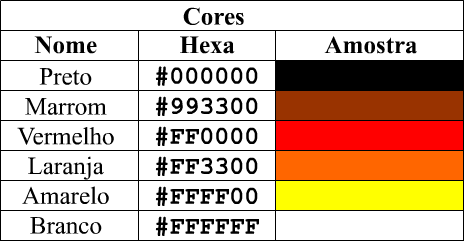
\includegraphics[scale=.7]{imagens/exemploQuadro}
		\\\textbf{Fonte:} Elaborada pelo autor
		\label{qua:exemplo}
	\end{quadro}
	\FloatBarrier
	
	
	Este é um exemplo de como usar equações. Referência cruzada: Equação~\ref{eq:exemplo}
	
	\begin{equation}
	\sum_{i=1}^{n} = \frac{n(n+1)}{2}
	\label{eq:exemplo}
	\end{equation}
	
	
	Exemplo de inserção de lista de código fonte (\textbf{\textcolor{red}{não use acentos no código!}}):
	
	\lstinputlisting[language=Java]{fontes/ClasseExemplo.java} 
	
	
	
	Este é um exemplo de como inserir texto sem formatação (ambiente verbatim):
	
	\begin{verbatim}
	Texto sem formatação, como espaçamento igual.
	\end{verbatim}
	
	
	Exemplo de lista de itens:
	
	\begin{itemize}
		\item \textbf{Item 1:} texto...;
		\item \textbf{Item 2:} texto...;
        \begin{itemize}
                \item \textbf{Subitem:} texto...;
                \item \textbf{Subitem:} texto...;
                \item \textbf{Subitem:} texto...;
            \end{itemize}
		\item \textbf{Item 3:} texto...;
		\item \textbf{Item n:} texto....
	\end{itemize}
	
	
	Exemplo de lista numerada:
	
	\begin{enumerate}
		\item \textbf{Item:} texto...;
		\item \textbf{Item:} texto...;
        \begin{enumerate}
            \item \textbf{Subitem:} texto...;
            \item \textbf{Subitem:} texto...;
            \item \textbf{Subitem:} texto...;
        \end{enumerate}
		\item \textbf{Item:} texto...;
		\item \textbf{Item:} texto....
	\end{enumerate}
	
	
	Exemplos de comandos para texto e referências:
	
	\begin{itemize}
		\item Para iniciar um novo parágrafo, basta deixar uma linha em branco no código fonte;
		\item Não force o compilador a pular mais de uma linha, pois terá influência negativa na composição do documento;
		\item Sempre deixe o \LaTeX\ realizar a formatação de parágrafos e posicionamento de elementos;
		\item Utilização de aspas simples (abertura \verb|`|, fechamento \verb|'|): `Texto entre aspas simples';
		\item Utilização de aspas duplas (abertura \verb|``|, fechamento \verb|''|): ``Texto entre aspas duplas'';
		\item Negrito (comando \verb|\textbf|): \textbf{texto em negrito};
		\item Itálico (comando \verb|\textit|): \textit{texto em itálico};
		\item Sublinhado (comando \verb|\underline|): \underline{texto sublinhado};
		\item Negrito e itálico (usar comandos juntos): \textbf{\textit{texto em negrito e itálico}};
		\item Alterar cor do texto (comando \verb|\textcolor{cor}{texto}|):
		\begin{itemize}
			\item Exemplo \verb|\textcolor{red}{texto}|: \textcolor{red}{texto vermelho};
			\item Exemplo \verb|\textcolor[RGB]{255, 102, 0}|: \textcolor[RGB]{255, 102, 0}{texto laranja};
			\item Exemplo \verb|\textcolor[HTML]{006AD7}|: \textcolor[HTML]{006AD7}{texto azul};
		\end{itemize}
		\item Ambiente matemático inline (comando \verb|$ expressão $|): $s = x^2-2x +1$;
		\item Referência normal (comando \verb|\cite|):
		\begin{itemize}
			\item \cite{Agaisse1995};
			\item \cite{Abedi2014};
			\item \cite{BtNomenclature2016};
		\end{itemize}
		\item Referência normal com mais de uma obra (comando \verb|\cite|):
		\begin{itemize}
			\item \cite{Agaisse1995, Abedi2014};
			\item \cite{Nelson2014, BtNomenclature2016, AgapitoTenfen2014};
		\end{itemize}
		\item Referência nome e ano (comando \verb|\citeauthorandyear|):
		\begin{itemize}
			\item \citeauthorandyear{Agaisse1995};
			\item \citeauthorandyear{Abedi2014};
			\item \citeauthorandyear{BtNomenclature2016};
		\end{itemize}
	\end{itemize}
	
	
	Exemplo 1 de referência direta:
	
	\begin{citacao}
		Os 20 aminoácidos usualmente encontrados como resíduos em proteínas contém um grupo $\alpha$-carboxil, um grupo $\alpha$-amino e um grupo R distinto substituído no átomo de carbono $\alpha$. O átomo de carbono $\alpha$ de todos os aminoácidos, com exceção da glicina, é assimétrico e, portanto, os aminoácidos podem existir em pelo menos duas formas estereoisoméricas. Somente os estereoisômeros L, com uma configuração relacionada à configuração absoluta da molécula de referência L-gliceraldeído, são encontrados em proteínas \cite[p. 81]{Nelson2014}
	\end{citacao}
	
	Exemplo 2 de referência direta:
	
	\begin{citacao}
		\textit{These various insecticidal proteins are synthesized during the stationary phase and accumulate in the mother cell as a crystal inclusion which can account for up to 25\% of the dry weight of the sporulated cells. The amount of crystal protein produced by a B. thuringiensis culture in laboratory conditions (about 0.5 mg of protein per ml) and the size of the crystals (24) indicate that each cell has to synthesize $10^6$ to $2 \times 10^6$ $\delta$-endotoxin molecules during the stationary phase to form a crystal} \cite[p. 1]{Agaisse1995}
	\end{citacao}
	
	Exemplo de nota de rodapé\footnote{Essa é uma nota de rodapé!}.
	
    
    
%%%%%%%%%%%%%%%%%%%%%%%%%%%%%%%%%%%%%%%%%%%%%%%%%%%%%%%%%%%%%%%%%%

	\section{Desenvolvimento}
    	
     Texto do desenvolvimento.
     
     
     
     %%%%%%%%%%%%%%%%%%%%%%%%%%%%%%%%%%%%%%%%%%%%%%%%%%%%%%%%%%%%%
     
     \subsection{Revisão da Literatura}
     
     Texto da revisão da literatura.
     
     
     
     %%%%%%%%%%%%%%%%%%%%%%%%%%%%%%%%%%%%%%%%%%%%%%%%%%%%%%%%%%%%%
     
     \subsection{Metodologia}
     
     Texto da metodologia.
     
     
     
     %%%%%%%%%%%%%%%%%%%%%%%%%%%%%%%%%%%%%%%%%%%%%%%%%%%%%%%%%%%%%
     
     
%%%%%%%%%%%%%%%%%%%%%%%%%%%%%%%%%%%%%%%%%%%%%%%%%%%%%%%%%%%%%%%%%%

	\section{Resultados e Discussão}
    	
     Texto dos resultados.
     
     
     
%%%%%%%%%%%%%%%%%%%%%%%%%%%%%%%%%%%%%%%%%%%%%%%%%%%%%%%%%%%%%%%%%%

	\section{Conclusões/Conclusões parciais}
	
	Texto das conclusões (as conclusões parciais são para a graduação na qualificação).
    
    
    
%%%%%%%%%%%%%%%%%%%%%%%%%%%%%%%%%%%%%%%%%%%%%%%%%%%%%%%%%%%%%%%%%%

	\section{Cronograma}
	
	Cronograma (para a graduação na qualificação).
	
	
	% ----------------------------------------------------------
	% ELEMENTOS PÓS-TEXTUAIS
	% ----------------------------------------------------------
	\postextual
	\bibliography{referencias}
	
	
\end{document}